% --- Memory anatomy of a training step ---
\begin{frame}{Where the Bytes Go}
  \begin{itemize}\itemsep0.35em
    \item[\textcolor{red}{$\blacktriangleright$}] GPU memory during training holds four things. Only the first is the model you think you are training.
      \begin{itemize}\itemsep0.15em\footnotesize
        \item \textbf{Parameters} $\Psi$ --- the weights used in the forward pass.
        \item \textbf{Gradients} --- one number per parameter, produced by the backward pass.
        \item \textbf{Optimizer states} --- Adam's two running moments plus the high-precision master copy of the weights.
        \item \textbf{Activations} --- everything the backward pass needs to re-read: layer inputs, attention scores, GeLU inputs, dropout masks.
      \end{itemize}
    \item[\textcolor{red}{$\blacktriangleright$}] The first three scale with \textbf{model size} and are called the \textbf{model states}. The fourth scales with \textbf{batch size $\times$ sequence length} and is called the \textbf{residual state}.
    \item[\textcolor{red}{$\blacktriangleright$}] The distinction matters because they are attacked by different tools: sharding for model states, recomputation and sequence splitting for activations.
  \end{itemize}
  \vspace{0.2em}
  {\scriptsize Terminology follows Rajbhandari et al., ``ZeRO: Memory Optimizations Toward Training Trillion Parameter Models,'' \href{https://arxiv.org/abs/1910.02054v3}{arXiv:1910.02054v3}, section \emph{Where Did All the Memory Go?}}
\end{frame}

\begin{frame}{The 16-Bytes-per-Parameter Rule}
  \begin{columns}[T,onlytextwidth]
    \column{0.53\textwidth}
      \footnotesize
      Mixed-precision training with Adam, per parameter:
      \vspace{0.3em}
      \begin{tabular}{@{}llr@{}}
        \toprule
        \textbf{Tensor} & \textbf{dtype} & \textbf{bytes} \\
        \midrule
        Weights (forward/backward)       & \texttt{bf16} & 2 \\
        Gradients                        & \texttt{bf16} & 2 \\
        \midrule
        Master copy of weights           & \texttt{fp32} & 4 \\
        Adam first moment $m$            & \texttt{fp32} & 4 \\
        Adam second moment $v$           & \texttt{fp32} & 4 \\
        \midrule
        \multicolumn{2}{@{}l}{\textbf{Total model states}} & \textbf{16} \\
        \bottomrule
      \end{tabular}
      \vspace{0.5em}
      \begin{itemize}\footnotesize\itemsep0.2em
        \item[\textcolor{red}{$\blacktriangleright$}] ZeRO writes this as $2\Psi + 2\Psi + K\Psi = 16\Psi$ bytes with the \textbf{optimizer multiplier} $K = 12$.
        \item[\textcolor{red}{$\blacktriangleright$}] \textbf{Assumptions:} Adam or AdamW; \texttt{fp32} optimizer states; one \texttt{fp32} master weight copy; gradients kept in \texttt{bf16}; activations counted separately.
      \end{itemize}
    \column{0.45\textwidth}
      \centering
      \vspace{0.8em}
      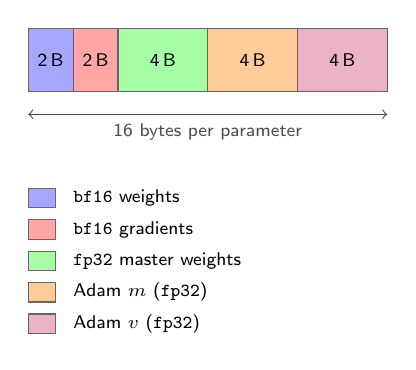
\begin{tikzpicture}[font=\sffamily\scriptsize, scale=0.95, every node/.style={transform shape}]
        % Bar: 16 bytes wide at 0.3 cm per byte. Offsets and widths are in bytes.
        \foreach \off/\wid/\col/\lab in {0/2/blue!35/{2\,B}, 2/2/red!35/{2\,B}, 4/4/green!35/{4\,B},
                                         8/4/orange!40/{4\,B}, 12/4/purple!30/{4\,B}} {
          \draw[fill=\col, draw=black!60] ({\off*0.3},0) rectangle ({(\off+\wid)*0.3},0.85);
          \node at ({(\off+\wid/2)*0.3},0.425) {\lab};
        }
        \draw[<->, black!70] (0,-0.3) -- (4.8,-0.3)
          node[midway, below, font=\sffamily\scriptsize] {16 bytes per parameter};
        \begin{scope}[shift={(0,-1.55)}]
          \foreach \col/\txt [count=\j from 0] in {blue!35/{\texttt{bf16} weights}, red!35/{\texttt{bf16} gradients},
              green!35/{\texttt{fp32} master weights}, orange!40/{Adam $m$ (\texttt{fp32})}, purple!30/{Adam $v$ (\texttt{fp32})}} {
            \draw[fill=\col, draw=black!60] (0,{-0.42*\j}) rectangle (0.36,{-0.42*\j+0.26});
            \node[anchor=west, font=\sffamily\scriptsize] at (0.48,{-0.42*\j+0.13}) {\txt};
          }
        \end{scope}
      \end{tikzpicture}\\[0.6em]
      {\scriptsize The green, orange, and purple blocks --- 12 of the 16 bytes --- are what ZeRO stage 1 shards first.}
  \end{columns}
\end{frame}

\begin{frame}[allowframebreaks]{Why fp32 Training Is Not Cheaper}
  \begin{itemize}\itemsep0.45em
    \item[\textcolor{red}{$\blacktriangleright$}] A common misconception: ``mixed precision halves training memory.'' It halves the \emph{activation} and \emph{gradient} memory, but the model-state total is unchanged.
    \item[\textcolor{red}{$\blacktriangleright$}] Pure \texttt{fp32} with Adam: weights $4$ + gradients $4$ + $m$ $4$ + $v$ $4$ = \textbf{16 bytes per parameter}.
    \item[\textcolor{red}{$\blacktriangleright$}] Mixed precision with Adam: $2 + 2 + 4 + 4 + 4$ = \textbf{16 bytes per parameter}.
    \item[\textcolor{red}{$\blacktriangleright$}] Both routes land on the same number, which is why ``$16\Psi$'' is the figure to memorise. Mixed precision buys \textbf{throughput} (tensor cores) and \textbf{activation memory}, not model-state memory.
    \item[\textcolor{red}{$\blacktriangleright$}] What \emph{does} move the number: a different optimizer. SGD with momentum is $2+2+4+4 = 12$ bytes; plain SGD is $8$; 8-bit Adam stores $m$ and $v$ in one byte each, giving $2+2+4+1+1 = 10$; and full-model \texttt{bf16} training without a master copy is $2+2+4+4 = 12$, at some risk to convergence.
    \item[\textcolor{red}{$\blacktriangleright$}] Parameter-efficient fine-tuning (LoRA) attacks the same term from the other side: if only 0.1\% of parameters carry gradients and optimizer states, $16\Psi$ collapses to roughly $2\Psi$ plus a rounding error.
  \end{itemize}
\end{frame}

\begin{frame}{Model States, by Model Size}
  \centering
  \footnotesize
  \begin{tabular}{@{}lrrrr@{}}
    \toprule
    \textbf{Model} & \textbf{Parameters $\Psi$} & \textbf{\texttt{bf16} weights} & \textbf{Model states $16\Psi$} & \textbf{80\,GB GPUs needed} \\
    \midrule
    GPT-2 XL     & $1.5 \times 10^{9}$   & 3\,GB    & 24\,GB    & 1 \\
    Llama-class  & $7 \times 10^{9}$     & 14\,GB   & 112\,GB   & 2 \\
    Llama-class  & $70 \times 10^{9}$    & 140\,GB  & 1.12\,TB  & 14 \\
    GPT-3        & $175 \times 10^{9}$   & 350\,GB  & 2.8\,TB   & 35 \\
    Llama-3 405B & $405 \times 10^{9}$   & 810\,GB  & 6.48\,TB  & 81 \\
    \bottomrule
  \end{tabular}
  \vspace{0.8em}
  \begin{itemize}\footnotesize\itemsep0.3em
    \item[\textcolor{red}{$\blacktriangleright$}] The last column is a \textbf{lower bound}: it counts model states only, at 100\% packing efficiency, with zero activations, zero fragmentation, and zero communication buffers. Real runs need more.
    \item[\textcolor{red}{$\blacktriangleright$}] Read it as the answer to ``how many GPUs before I can even start?'' --- not ``how many GPUs should I use?''
    \item[\textcolor{red}{$\blacktriangleright$}] Note the asymmetry with inference: serving the 70B model needs 140\,GB of weights (2 GPUs), training it needs 1.12\,TB (14 GPUs). \textbf{Training is roughly 8$\times$ the memory of inference} for the same model.
  \end{itemize}
\end{frame}

\begin{frame}{Activations: the Term That Depends on Your Batch}
  \begin{itemize}\footnotesize\itemsep0.35em
    \item[\textcolor{red}{$\blacktriangleright$}] Model states are fixed once you pick the model. \textbf{Activations are the term you control} --- and the term that explodes with long context.
    \item[\textcolor{red}{$\blacktriangleright$}] For a standard transformer layer in mixed precision, with micro-batch $b$, sequence length $s$, hidden size $h$, and $a$ attention heads, Korthikanti et al.\ count the stored activations exactly:
      \[
        \text{bytes per layer} \;=\; s\,b\,h\left(34 + \frac{5\,a\,s}{h}\right).
      \]
    \item[\textcolor{red}{$\blacktriangleright$}] The $34$ collects the LayerNorm, QKV, linear-layer and GeLU inputs, the stored $Q$, $K$ and $V$, and the dropout masks. The $5as/h$ term is the \textbf{materialised $s \times s$ attention matrix}: the only piece that is quadratic in sequence length.
    \item[\textcolor{red}{$\blacktriangleright$}] \textbf{Worked example}, a 7B-class model with $h = 4096$, $a = 32$, $L = 32$, $s = 2048$, micro-batch $b = 1$:
      \[
        \tfrac{5as}{h} = 80, \quad sbh(34+80) = 8.39\times10^{6} \cdot 114 \approx 0.96\ \text{GB/layer}, \quad \times\,32 \approx \mathbf{31\ GB}.
      \]
    \item[\textcolor{red}{$\blacktriangleright$}] Total for one step: $112 + 31 = \mathbf{143\ GB}$ on a card with 80\,GB. Even a micro-batch of \emph{one} does not fit.
  \end{itemize}
  \vspace{0.1em}
  {\scriptsize Equation 1 of Korthikanti et al., \href{https://arxiv.org/abs/2205.05198v1}{arXiv:2205.05198v1}, Section 4.1.}
\end{frame}

\begin{frame}{Two Things That Make Activations Worse, and One That Helps}
  \begin{itemize}\itemsep0.4em
    \item[\textcolor{red}{$\blacktriangleright$}] \textbf{Longer context is superlinear.} Take the same 7B model to $s = 8192$: the quadratic term becomes $5as/h = 320$, so each layer costs $sbh(34+320) \approx 11.9$\,GB and the stack costs $\approx 380$\,GB --- a $4\times$ longer sequence for a $12\times$ memory bill.
    \item[\textcolor{red}{$\blacktriangleright$}] \textbf{Bigger micro-batches are linear.} Activations scale exactly with $b$, which is why the first thing that fails when you raise the batch size is memory, not compute.
    \item[\textcolor{red}{$\blacktriangleright$}] \textbf{IO-aware attention removes the quadratic term.} FlashAttention never materialises the $s \times s$ matrix, so the $5as/h$ term disappears and the per-layer cost drops to $34sbh$. The stack then costs $9.1$\,GB instead of $31$\,GB at $s = 2048$, and $36$\,GB instead of $380$\,GB at $s = 8192$.
    \item[\textcolor{red}{$\blacktriangleright$}] FlashAttention and FlashAttention-2 are covered earlier; here we only need the consequence, which is that the \emph{linear} $34sbh$ term is what distributed training has to deal with, and it is still large.
  \end{itemize}
\end{frame}

\begin{frame}{Activation Recomputation (Gradient Checkpointing)}
  \begin{columns}[T,onlytextwidth]
    \column{0.55\textwidth}
      \begin{itemize}\footnotesize\itemsep0.35em
        \item[\textcolor{red}{$\blacktriangleright$}] \textbf{The trade.} Do not store the intermediate activations. Store only the \emph{input} to each transformer layer, and recompute the interior with an extra forward pass when the backward pass reaches it.
        \item[\textcolor{red}{$\blacktriangleright$}] \textbf{Full recomputation} at layer granularity reduces the whole activation term to $2 s b h L$ bytes. For our 7B example that is $2 \cdot 2048 \cdot 4096 \cdot 32 \approx 0.54$\,GB, down from 31\,GB --- a $57\times$ reduction.
        \item[\textcolor{red}{$\blacktriangleright$}] \textbf{The price} is one extra forward pass (Chen et al.): about 33\% more compute in theory, and Megatron's authors measure \textbf{30--40\% execution-time overhead} on real training runs.
        \item[\textcolor{red}{$\blacktriangleright$}] \textbf{Selective recomputation} recomputes only the cheap-but-huge pieces (the attention softmax and dropout region) and stores the rest. It recovers over 90\% of the lost time while keeping most of the memory saving.
        \item[\textcolor{red}{$\blacktriangleright$}] In PyTorch this is \texttt{torch.utils.checkpoint}; in Hugging Face, \texttt{model.gradient\_checkpointing\_enable()}.
      \end{itemize}
    \column{0.43\textwidth}
      \centering
      \vspace{0.6em}
      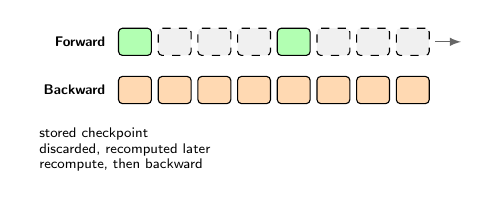
\begin{tikzpicture}[font=\sffamily\scriptsize, >=latex, scale=0.72,
          every node/.style={transform shape},
          lay/.style={draw, minimum width=0.58cm, minimum height=0.48cm, rounded corners=0.05cm},
          kept/.style={lay, fill=green!30},
          drop/.style={lay, fill=gray!12, dashed},
          redo/.style={lay, fill=orange!30}]
        \node[font=\sffamily\scriptsize, anchor=east] at (-0.4,0.9) {\textbf{Forward}};
        \node[kept] at (0,0.9) {}; \node[drop] at (0.7,0.9) {};
        \node[drop] at (1.4,0.9) {}; \node[drop] at (2.1,0.9) {};
        \node[kept] at (2.8,0.9) {}; \node[drop] at (3.5,0.9) {};
        \node[drop] at (4.2,0.9) {}; \node[drop] at (4.9,0.9) {};
        \draw[->, black!60] (5.3,0.9) -- (5.75,0.9);
        \node[font=\sffamily\scriptsize, anchor=east] at (-0.4,0.05) {\textbf{Backward}};
        \foreach \x in {0, 0.7, 1.4, 2.1, 2.8, 3.5, 4.2, 4.9} {\node[redo] at (\x,0.05) {};}
        \node[anchor=west, font=\sffamily\scriptsize, align=left] at (-1.9,-1.0)
          {\textcolor{green!45!black}{$\blacksquare$}~stored checkpoint\\
           \textcolor{gray}{$\blacksquare$}~discarded, recomputed later\\
           \textcolor{orange!70!black}{$\blacksquare$}~recompute, then backward};
      \end{tikzpicture}\\[0.5em]
      {\scriptsize Store one activation per boundary; rebuild the rest on demand.}
  \end{columns}
\end{frame}

\begin{frame}{Gradient Accumulation: a Bigger Batch Without More Memory}
  \begin{itemize}\footnotesize\itemsep0.4em
    \item[\textcolor{red}{$\blacktriangleright$}] Large-model training wants a \textbf{global batch} of millions of tokens for stable optimisation, but activation memory caps the \textbf{micro-batch} you can fit on one device.
    \item[\textcolor{red}{$\blacktriangleright$}] \textbf{Gradient accumulation} decouples them: run $m$ micro-batches, sum their gradients into the same buffer, and step the optimizer once.
      \[
        \text{global batch} \;=\; \underbrace{b}_{\text{micro-batch}} \times \underbrace{m}_{\text{accumulation steps}} \times \underbrace{d}_{\text{data-parallel ranks}}
      \]
    \item[\textcolor{red}{$\blacktriangleright$}] Memory cost: \textbf{zero}. The gradient buffer already exists; only one micro-batch of activations is live at a time.
    \item[\textcolor{red}{$\blacktriangleright$}] Time cost: also close to zero, \emph{provided} you skip the all-reduce on the intermediate micro-batches. PyTorch DDP exposes this as the \texttt{no\_sync()} context manager; forgetting it multiplies your communication bill by $m$.
    \item[\textcolor{red}{$\blacktriangleright$}] Watch the loss normalisation: divide by $m$ (or use \texttt{mean} reduction consistently), or your effective learning rate silently scales with the accumulation count.
    \item[\textcolor{red}{$\blacktriangleright$}] The same $m$ reappears in pipeline parallelism as the \textbf{number of micro-batches}, where it controls the pipeline bubble. It is the single most reused hyperparameter in this lecture.
  \end{itemize}
\end{frame}
